\newpage
\section{Introduzione Maching Learning}
Questo per molti è un nuovo vampo, con una metodologia diversa di approccio. Infatti qui gli algoritmi non vengono usati
per risolvere un problema ma invece per creare modelli dai dati.\\
Con "Learning" (apprendimento) si intende i principi universali per gli essere viventi, la società e le macchine:\\\\
\textit{Il problema dell’apprendimento è senza dubbio al centro stesso del problema intelligenza, sia biologica che artificiale (Poggio, Shelton, AI Magazine 1999)}\\\\
Il "Learning" è quindi un obiettivo complesso, ed un campo di ricerca in continua crescita.
Il \textbf{Il machine learning} è emersa come un’area di ricerca combinata l'obiettivo di creare computer in grado di apprendere (IA) e nuovi potenti strumenti adattivi/statistici con basi rigorose scienza computazional.\\
Macchine che imparano da sole. Perché? Lusso o necessità?
\begin{itemize}
    \item Crescente disponibilità e necessità di analisi di dati empirici.
    \item Difficile fornire adattività/intelligenza mediante la programmazione.
\end{itemize}
Gli obbiettivi principali del ML includono:
\begin{itemize}
    \item Come metodologia AI, costruisci sistemi intelligenti adattivi (Dal motore di ricerca alla robotica ...).
    \item Come apprendimento statistico, costruisci un potente sistema predittivo per l'analisi intelligente dei dati (strumenti per il “data scientist”).
    \item Come metodo informatico per ambiti applicativi innovativi, usare modelli come tool per problemi complessi, interdisciplinari (dalla analisi di dati biologici per capire immagini).
\end{itemize}
Noi in particolare andiamo a studiare il ML perché è un'opportunità per conoscere \textbf{nuovi paradigmi informatici}, con un approccio diverso rispetto a alla programmazione standard, IA algoritmica/classica approcci. 
Tipico dell'area del soft computing/intelligenza computazionale. Per trovare soluzioni approssimative per problemi difficili, difficile da formalizzare
per algoritmo "fatto a mano". Costruire nuovi \textbf{sistemi intelligenti} robusti e ampiamente applicabili.
\begin{figure}[h!]
    \centering
    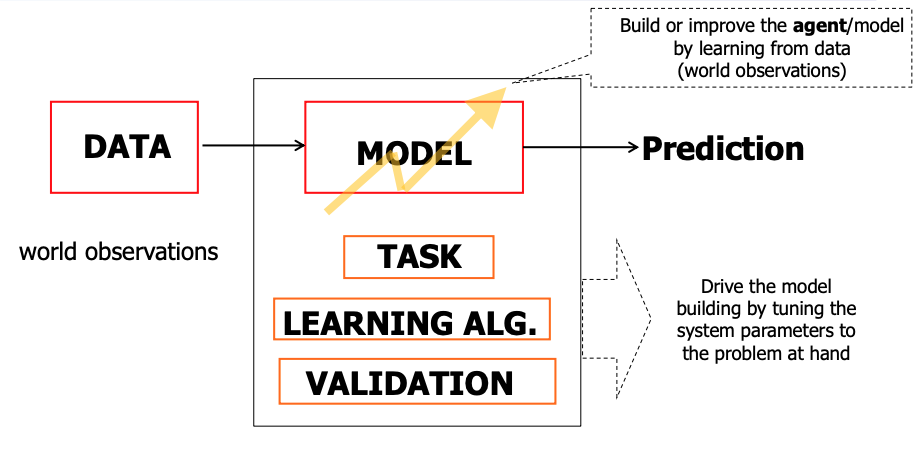
\includegraphics[width=0.65\textwidth]{images/ml-overview.png}
\end{figure}
\begin{example}
    Un esempio potrebbe essere riconoscere dei numeri scritti a mano.
    \begin{itemize}
        \item \textbf{Input}: abbiamo un insieme di immagini di numeri scritti a mano.
        \item \textbf{Problem}: costruire un modello che riceve come input un immagine di un numero scritto a mano e capisce che numero è.
    \end{itemize}
    La difficoltà qui sta nel \textbf{formalizzare} esattamente la soluzione del problema: infatti ci potrebbe essere
    la presenza di \textbf{"rumore"} e \textbf{ambiguità} dei dati.
\end{example}
\subsection{Apprendimento supervisionato}
Questo problema rientra nell'insieme del \textbf{Supervised learning} (classificazione, regressione).
\begin{figure}[h!]
    \centering
    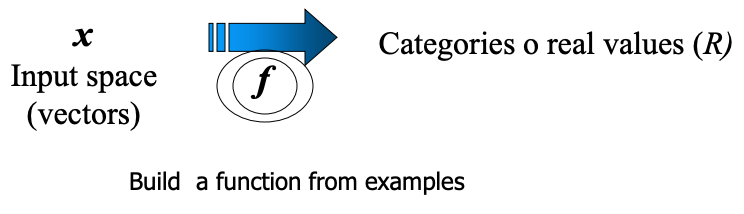
\includegraphics[width=0.65\textwidth]{images/sup-learning.png}
\end{figure}
Nel apprendimento supervisionato abbiamo che:
\begin{itemize}
    \item \textbf{Given}: vengono dati degli esempi di allenamento $<input, outpu> = (x,d)$, per una funzione sconosciuta $f$.
    Il \textbf{target value} è il valore desiderato $d$ o $t$ o $y$ ... viene fornito dall'insegnamento secondo $f(x)$ per etichettare i dati.
    \item \textbf{Find}: viene trovato una buona approssimazione di $f$.
\end{itemize}
Come abbiamo già detto prima l'apprendimento supervisionato di divide in \textbf{classificazione} e \textbf{regressione}.
\begin{definition}[Classificazione]
   $f(x)$ ritorna (la presunta) classe di correttezza per $x$, $f(x)$ è funzione a valori discreti $\in \{1, 2, \dots, k\}$.   
\end{definition}
\begin{definition}[Regressione]
    Valori di uscita conitnui reali (approssimare una funzione target a valore reale, in $R, R^*$)
\end{definition}

\subsection{Apprendimento non supervisionato}
\begin{definition}[Training Set (TS)]
    Insieme di dati senza etichetta.
\end{definition}
Per esempio. Per trovare raggruppamenti naturali in un insieme di dati (clustering,
Riduzione dimensionale/Visualizzazione/Preelaborazione, modellazione della densità di dati.).
\begin{figure}[h!]
    \centering
    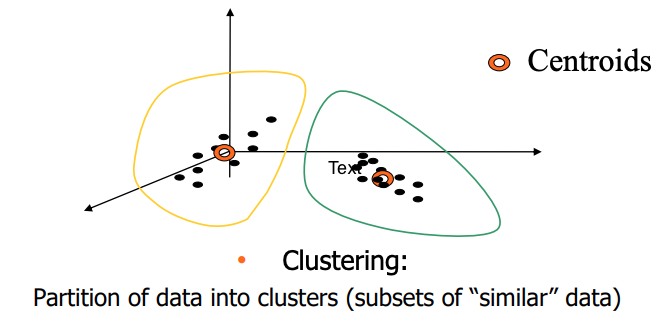
\includegraphics[width=0.65\textwidth]{images/unsupervides-learning.png}
\end{figure}

\subsection{Model}
Un \textbf{modello} ha l'obbiettivo di catturare/descrivere le relazioni tra i dati (sul base del compito). 
Va anche a definire la classe di funzioni che la macchina che apprende può eseguire implementare (spazio delle ipotesi)
\begin{example}
    Un insieme di funzioni $h(x, w)$ dove $w$ sono dei paramentri (astratti).
\end{example}
Altre definizioni importanti da dire sono le seguenti:
\begin{itemize}
    \item \textbf{Training example}: un esempio delle forma $(x, f(x) + noise)$ con $x$ che solitamente 
    è un vettore di caratteristiche, (d o t) $y = f(x) + noise$ è chiamato il valore target.
    \item \textbf{Target function}: la vera funzione $f$.
    \item \textbf{Ipotesi}: Una funzione proposta h ritenuta simile a f. Un espressione in un dato linguaggio che descrive le relazioni tra i dati.
    \item \textbf{Spazio di ipotesi}: Lo spazio di tutte le ipotesi (modelli specifici) che può, in linea di principio, essere prodotto dall'algoritmo di apprendimento.
\end{itemize}
Fortunatamente già conoscete alcuni linguaggi in cui esprimere relazioni che possiamo usare per esprimere modelli di ML (le ipotesi h):
\begin{itemize}
    \item \textbf{Logica} (proposizionale)
    \item \textbf{Equazioni numeriche}
    \item \textbf{Probabilità}: questo verrà reintrodotto per la rappresentazione della conoscenza incerta in AI (e quindi per esprimere modelli di ML)
\end{itemize}
Una prima vista dei differenti modi in cui verranno rappresentate le ipotesi.
\begin{itemize}
    \item \textbf{Liner models}
    \item \textbf{Symbolic rules}: (lo spazio delle ipotesi è basato sulla rappresentazione discreta); sono possibili regole diverse, ad ess:
    \begin{lstlisting}
        if(x1 = 0) and (x2 = 1) then h(x) = 1
        else h(x) = 0
    \end{lstlisting}
    \item \textbf{Probabilistic models}: una stima $p(x,y)$
\end{itemize}

\subsection{Learning algorithms}
Basandosi su dati, attività e modello, apprendimento come ricerca (euristica) attraverso lo spazio delle ipotesi H di l'ipotesi migliore.
Cioè la migliore approssimazione alla funzione target (sconosciuta). Tipicamente ricercando la h con il minimo “errore”.
\begin{example}
    Per esempio i paramentri liveri del modello sono adattati al compito da svolgere, per esempio
    migliore $w$ nei modelli lineari, migliori regole per i modelli simbolici, ecc.
\end{example}
\hspace{-15pt}$H$ potrebbe non coincidere con l'insieme di tutte le possibili funzioni e la ricerca
non può essere esaustiva: occore fare delle ipotesi, noi vedremo il ruolo del bias induttivo.
\begin{figure}[h!]
    \centering
    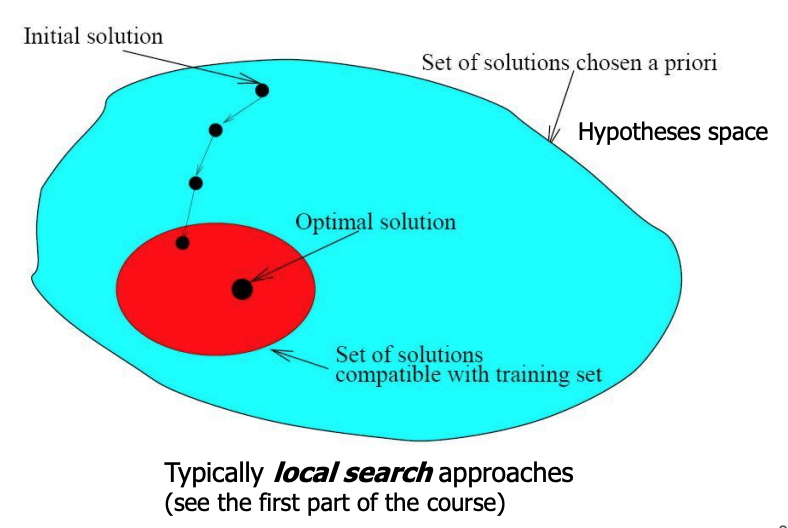
\includegraphics[width=0.5\textwidth]{images/learning-algo.png}
\end{figure}
\hspace{-15pt}\textbf{Apprendimento}: cercare una \textbf{buona funzione} in una funzione
spazio dai dati noti (in genere riducendo al minimo un errore/perdita).
\begin{definition}
    \textbf{Buon} w.r.t. errore di generalizzazione: misura come
    il modello prevede con precisione su nuovi campioni di dati
    (Errore/perdita misurata su nuovi dati) (errore basso, alta precisione e viceversa)
\end{definition}
\hspace{-15pt}La generalizzazione è un punto cruciale nel ML. Essa comprende:
\begin{itemize}
    \item \textbf{Fase di apprendimento}(formazione, adattamento): costruire il modello
    dai dati conosciutidati di addestramento (e bias)
    \item \textbf{Fase predittiva} (test): applicare a nuovi esempi (prendiamo gli input x’; calcoliamo la risposta secondo il modello; confrontiamo con il suo bersaglio che il modello non ha mai visto).
    Valutazione dell’ipotesi predittiva, cioè del \textbf{capacità di generalizzazione}.
    \item \textbf{Teoria}: Per esempio. Teoria dell'apprendimento statistico. In quali condizioni (matematiche) un modello è in grado di farlo generalizzare?
\end{itemize}
\begin{note}
    Le performance in ML sono uguali all'accuratezza nelle previsioni, stimato dall'errore calcolato sul set di test (Hold out).
\end{note}